\documentclass[10pt,reprint]{sigplanconf}
\usepackage{times}
\usepackage{amssymb,amsmath}
\usepackage{ifxetex,ifluatex}
\usepackage{fixltx2e} % provides \textsubscript
\ifnum 0\ifxetex 1\fi\ifluatex 1\fi=0 % if pdftex
  \usepackage[T1]{fontenc}
  \usepackage[utf8]{inputenc}
\else % if luatex or xelatex
  \ifxetex
    \usepackage{mathspec}
    \usepackage{xltxtra,xunicode}
  \else
    \usepackage{fontspec}
  \fi
  \defaultfontfeatures{Mapping=tex-text,Scale=MatchLowercase}
  \newcommand{\euro}{€}
\fi
% use upquote if available, for straight quotes in verbatim environments
\IfFileExists{upquote.sty}{\usepackage{upquote}}{}
% use microtype if available
\IfFileExists{microtype.sty}{%
\usepackage{microtype}
\UseMicrotypeSet[protrusion]{basicmath} % disable protrusion for tt fonts
}{}
\usepackage{color}
\usepackage{fancyvrb}
\newcommand{\VerbBar}{|}
\newcommand{\VERB}{\Verb[commandchars=\\\{\}]}
\DefineVerbatimEnvironment{Highlighting}{Verbatim}{commandchars=\\\{\}}
% Add ',fontsize=\small' for more characters per line
\usepackage{framed}
\definecolor{shadecolor}{RGB}{248,248,248}
\newenvironment{Shaded}{\begin{snugshade}}{\end{snugshade}}
\newcommand{\KeywordTok}[1]{\textcolor[rgb]{0.13,0.29,0.53}{\textbf{{#1}}}}
\newcommand{\DataTypeTok}[1]{\textcolor[rgb]{0.13,0.29,0.53}{{#1}}}
\newcommand{\DecValTok}[1]{\textcolor[rgb]{0.00,0.00,0.81}{{#1}}}
\newcommand{\BaseNTok}[1]{\textcolor[rgb]{0.00,0.00,0.81}{{#1}}}
\newcommand{\FloatTok}[1]{\textcolor[rgb]{0.00,0.00,0.81}{{#1}}}
\newcommand{\CharTok}[1]{\textcolor[rgb]{0.31,0.60,0.02}{{#1}}}
\newcommand{\StringTok}[1]{\textcolor[rgb]{0.31,0.60,0.02}{{#1}}}
\newcommand{\CommentTok}[1]{\textcolor[rgb]{0.56,0.35,0.01}{\textit{{#1}}}}
\newcommand{\OtherTok}[1]{\textcolor[rgb]{0.56,0.35,0.01}{{#1}}}
\newcommand{\AlertTok}[1]{\textcolor[rgb]{0.94,0.16,0.16}{{#1}}}
\newcommand{\FunctionTok}[1]{\textcolor[rgb]{0.00,0.00,0.00}{{#1}}}
\newcommand{\RegionMarkerTok}[1]{{#1}}
\newcommand{\ErrorTok}[1]{\textbf{{#1}}}
\newcommand{\NormalTok}[1]{{#1}}

\DefineVerbatimEnvironment{Highlighting}{Verbatim}{commandchars=\\\{\},fontsize=\scriptsize}

\usepackage{graphicx}
\makeatletter
\def\maxwidth{\ifdim\Gin@nat@width>\linewidth\linewidth\else\Gin@nat@width\fi}
\def\maxheight{\ifdim\Gin@nat@height>\textheight\textheight\else\Gin@nat@height\fi}
\makeatother
% Scale images if necessary, so that they will not overflow the page
% margins by default, and it is still possible to overwrite the defaults
% using explicit options in \includegraphics[width, height, ...]{}
\setkeys{Gin}{width=\maxwidth,height=\maxheight,keepaspectratio}
\ifxetex
  \usepackage[setpagesize=false, % page size defined by xetex
              unicode=false, % unicode breaks when used with xetex
              xetex]{hyperref}
\else
  \usepackage[unicode=true]{hyperref}
\fi
\hypersetup{breaklinks=true,
            bookmarks=true,
            pdfauthor={},
            pdftitle={Tackling the Reproducibility Problem in Systems Research with Declarative Experiment Specifications},
            colorlinks=true,
            citecolor=blue,
            urlcolor=blue,
            linkcolor=magenta,
            pdfborder={0 0 0}}
\urlstyle{same}  % don't use monospace font for urls
\renewcommand*{\hyperref}[2][\ar]{\def\ar{#2}#2\autoref{#1}}
\renewcommand*{\figureautorefname}{Figure}
\renewcommand*{\sectionautorefname}{Section}
\renewcommand*{\subsectionautorefname}{Section}
\renewcommand*{\subsubsectionautorefname}{Section}
% Make links footnotes instead of hotlinks:
\renewcommand{\href}[2]{#2\footnote{\url{#1}}}
% no spacing just use whatever has been defined somewhere else
\setcounter{secnumdepth}{5}

% a0poster {
% }



% title {
  \title{Tackling the Reproducibility Problem in Systems Research with
Declarative Experiment Specifications}
      % }


% authors {
 \authorinfo{Ivo Jimenez, Carlos Maltzahn}{UC Santa Cruz}{\texttt{\{ivo,carlosm\}@cs.ucsc.edu}}  \authorinfo{Jay Lofstead}{Sandia National Lab}{\texttt{gflofst@sandia.gov}}  \authorinfo{Adam Moody, Kathryn Mohror}{Lawrence Livermore National Lab}{\texttt{\{moody20,kathryn\}@llnl.gov}}  \authorinfo{Remzi Arpaci-Dusseau, Andrea Arpaci-Dusseau}{UW Madison}{\texttt{\{dusseau,remzi\}@cs.wisc.edu}} 
% }

\date{}


% letter {
% }

\begin{document}

% a0poster {
% }

\maketitle

% a0poster {
% }

\begin{abstract}
Validating experimental results in the field of computer systems is a
challenging task, mainly due to the many changes in software and
hardware that computational environments go through. Determining if an
experiment is reproducible entails two separate tasks: re-executing the
experiment and validating the results. Existing reproducibility efforts
have focused on the former, envisioning techniques and infrastructures
that make it easier to re-execute an experiment. In this work we focus
on the latter by analyzing the validation workflow that an experiment
re-executioner goes through. We notice that validating results is done
on the basis of experiment design and high-level goals, rather than
exact quantitative metrics. Based on this insight, we introduce a
declarative format for specifying the high-level components of an
experiment as well as describing generic, testable conditions that serve
as the basis for validation. We present a use case in the area of
storage systems to illustrate the usefulness of this approach. We also
discuss limitations and potential benefits of using this approach in
other areas of experimental systems research.
\end{abstract}

\category{D.3.2}{Language Classifications}{Very high-level languages}
\category{D.4.m}{Operating Systems}{Miscellaneous}
\category{K.7.3}{The Computing Profession}{General}


\keywords  reproducibility

% a0poster {
% }


% letter {
% }


\section{Introduction}\label{introduction}

A key component of the scientific method is the ability to revisit and
reproduce previous experiments. Registering detailed information about
an experiment allows scientists to understand and validate results.
Reproducibility also plays a major role in education since a student can
learn by looking at provenance information, re-evaluate the questions
that the original experiment answered and thus ``stand on the shoulder
of giants''.

The role of computers in new scientific discoveries has only increased
and will continue. Coupled with this, the advent of cloud computing
offers new opportunities for experiment validation. Cloud computing
makes it easier to share code and data simplifying collaboration for
implementing experiments. While it is becoming easier to collaborate,
the same cannot be said about experiment validation. There is a serious
lack of tools that help researchers identify when an experiment is
reproducible. The goal of our work is to close this gap in the area of
systems research and storage systems in particular. In systems research,
performance \emph{is} the subject of study and we need to look at it as
a primary issue. As a consequence, repeating an experiment with the
expectation of obtaining exact same results is unrealistic and further
complicates the reproducibility problem.

When discussing reproducibility, the terms \emph{reproducibility},
\emph{repeatability}, \emph{replicability} and \emph{recomputability}
(among many others) are often used, sometimes interchangeably. In our
work we only employ \emph{repeatability} and \emph{reproducibility}. We
borrow the definitions introduced by Vitek et al. {[}1{]}:

\begin{quote}
Repeatability. \emph{The ability to re-run the exact same experiment
with the same method on the same or similar system and obtain the same
or very similar result.}

Reproducibility. \emph{The independent confirmation of a scientific
hypothesis through reproduction by an independent researcher/lab. The
reproductions are carried out after a publication, based on the
information in the paper and possibly some other information, such as
data sets, published via scientific data repositories or provided by the
authors on inquiry}.
\end{quote}

While desirable, it is impractical to assume that the exact same
experiment can be run on the same or a similar system, thus our main
focus is reproducibility. Today's computational environments undergo a
continual stream of changes that make it difficult for an experiment to
observe the same state across multiple executions. Version-control
systems (VCS) are sometimes used to ease the recreation of an
experimental environment. Having a specific version ID for the source
code and data associated with an article on a public repository
significantly reduces the burden of recreating the means of an
experiment {[}2{]}. However, availability of the source code does not
guarantee reproducibility {[}3{]} since the code might not compile and,
even if compilable, the resulting program might not generate the same
results. Recreating an environment that resembles the one where an
experiment was originally executed is a challenging task {[}4{]}.
Virtualization technologies can play a big role in accomplishing this
{[}5,6{]}. In the end, the re-implementation of an experiment might be
audited by experts to confirm that they resemble the original.

The reproduction of an experiment can be seen as being composed of (1)
its execution and (2) the validation of the results. Generally, these
two tasks are conflated when designating an experiment as reproducible.
In our case, we treat them separately and focus on the latter. At this
stage, the reviewer has to answer the question: \emph{``are the
re-generated results validating the original ones?''} An alternative but
problematic validation criterion can rely on the exact quantitative
observations, that is, results validate the original work if the exact
same numerical values of the original output are obtained. This leaves
little leeway for validation since more often than not an experiment
will get executed on environments that differ from the original.

Thus, ideally, we would like to have a way of specifying validation
criteria that are as independent as possible from the particular
implementation details, i.e., a way of testing the validity of the
original work that is agnostic to the implementation of the experiment.
A potential solution is to have an experiment specification that
describes the expected outcome in abstract rather than absolute terms.
We propose to take experiment goals as the basis for validation and
treat quantitative observations in the context of these goals.

\hyperdef{}{sec:goals-means-obs}{\section{Goals, Means, and
Observations}\label{sec:goals-means-obs}}

The high-level structure of an experiment can be described as having
three components: goals, means, and observations. Two additional
transient components, output data and result visualizations, are created
as part of running the experiment and are used as a basis for
observations (Figure 1).

\begin{figure}[htbp]
\centering
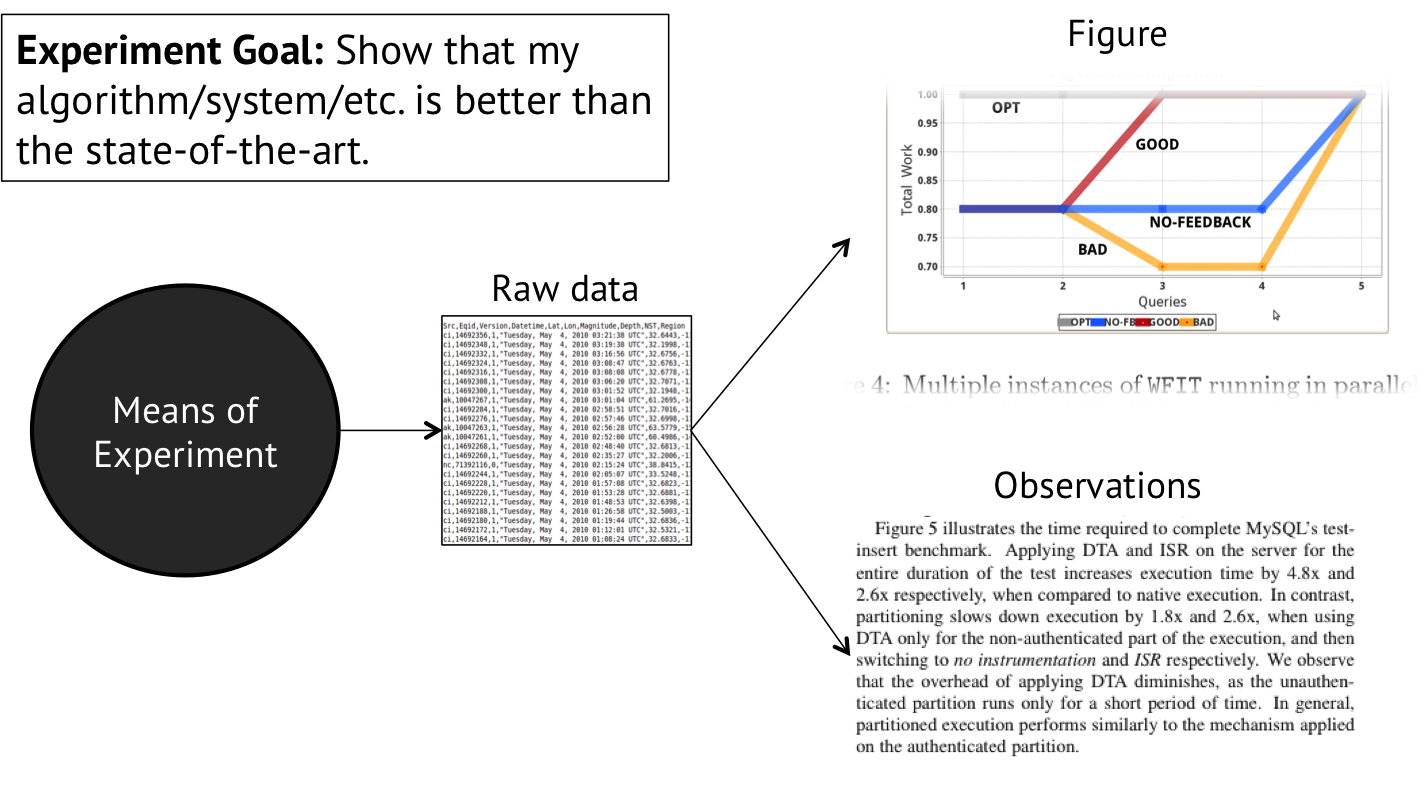
\includegraphics{figures/goals.png}
\caption{High-level structure of an experiment.}
\end{figure}

\textbf{Goals}: An experiment is designed with a particular goal in
mind, for example, to show that under certain circumstances, a new
system or algorithm improves the state-of-the-art by an order of
magnitude.

\textbf{Means}: An experiment is composed of a relatively complex
computational environment that includes one or more of the following:
hardware, virtualization, OS, configuration, code, data and workload. We
refer to these as the means of the experiment and use this term to
denote the particularities of how the experimental environment and
procedures are carried out.

\textbf{Observations}: As part of the experiment execution, metrics are
collected into an output dataset. This raw data can optionally be
summarized (e.g., with statistical descriptors) before being displayed
in a figure and described in the form of observations made in the prose
of the article. The observations made about the output data properties
are the basis on which an author proves and corroborates the hypothesis
of her work.

A declarative format provides a way to express, at a high-level, the
relationship among the goals and means of an experiment, the raw data it
produces, and the figures and observations discussed in the article. In
other words, it enables the author to provide an experiment design
description, its means of execution, and the expected observations that
validate the author's claims. Such a description serves two purposes.
First, a reviewer or reader with access to this description can, on her
own, validate the original work by testing whether the original
observations hold on the re-generated output data. Secondly, the
explicit specification of these high-level elements aid an author in
enhancing the design and presentation of the experimental evaluation of
a system by forcing her to think about all aspects of the experiment
rather than just generating results for a paper.

\hyperdef{}{sec:format}{\section{Experiment Specification
Format}\label{sec:format}}

An experiment specification format (ESF) allows a scientist to
explicitly and declaratively capture an experiment's high-level
structure. An example JSON file is shown below. It corresponds to a
simplified version of the specification of a published experiment
(\hyperref[sec:case]{see~}). We describe each section of the ESF next.

\begin{Shaded}
\begin{Highlighting}[numbers=left,,]
\FunctionTok{\{}
  \DataTypeTok{"goal_location"}\FunctionTok{:} \FunctionTok{\{}
     \DataTypeTok{"sec"}\FunctionTok{:} \StringTok{"6.1"}\FunctionTok{,}
     \DataTypeTok{"par"}\FunctionTok{:} \DecValTok{5}
  \FunctionTok{\},}
  \DataTypeTok{"goal_text"}\FunctionTok{:} \StringTok{"demonstrate that Ceph scales linearly}
\StringTok{     with the size of the cluster"}\FunctionTok{,}
  \DataTypeTok{"goal_category"}\FunctionTok{:} \OtherTok{[}\StringTok{"proof_of_concept"}\OtherTok{]}\FunctionTok{,}
  \DataTypeTok{"experiments"}\FunctionTok{:}\OtherTok{[} \FunctionTok{\{}
     \DataTypeTok{"reference"}\FunctionTok{:}\StringTok{"figure-8"}\FunctionTok{,}
     \DataTypeTok{"name"}\FunctionTok{:}\StringTok{"scalability experiment"}\FunctionTok{,}
     \DataTypeTok{"tags"}\FunctionTok{:}\OtherTok{[}\StringTok{"throughput"}\OtherTok{]}\FunctionTok{,}
     \DataTypeTok{"hardware_dependencies"}\FunctionTok{:} \OtherTok{[}\FunctionTok{\{}
        \DataTypeTok{"type"}\FunctionTok{:} \StringTok{"hdd"}\FunctionTok{,}
        \DataTypeTok{"bw"}\FunctionTok{:} \StringTok{"58MB/s"}
     \FunctionTok{\}}\OtherTok{,} \FunctionTok{\{}
        \DataTypeTok{"type"}\FunctionTok{:} \StringTok{"network"}\FunctionTok{,}
        \DataTypeTok{"bw"}\FunctionTok{:} \StringTok{"1GbE"}
     \FunctionTok{\}}\OtherTok{]}\FunctionTok{,}
     \DataTypeTok{"software_dependencies"}\FunctionTok{:} \OtherTok{[}\FunctionTok{\{}
       \DataTypeTok{"type"}\FunctionTok{:} \StringTok{"os"}\FunctionTok{,}
       \DataTypeTok{"kernel"}\FunctionTok{:} \StringTok{"linux 2.6.32"}\FunctionTok{,}
       \DataTypeTok{"distro"}\FunctionTok{:} \StringTok{"debian 6.0"}
     \FunctionTok{\}}\OtherTok{,} \FunctionTok{\{}
       \DataTypeTok{"type"}\FunctionTok{:} \StringTok{"storage"}\FunctionTok{,}
       \DataTypeTok{"name"}\FunctionTok{:} \StringTok{"ceph"}\FunctionTok{,}
       \DataTypeTok{"version"}\FunctionTok{:} \StringTok{"0.1.67"}
     \FunctionTok{\}}\OtherTok{]}\FunctionTok{,}
     \DataTypeTok{"workload"}\FunctionTok{:} \FunctionTok{\{}
       \DataTypeTok{"type"}\FunctionTok{:} \StringTok{"rados-benchmark"}\FunctionTok{,}
       \DataTypeTok{"configuration"}\FunctionTok{:} \OtherTok{[}
         \StringTok{"object-size"}\ErrorTok{:} \StringTok{"4mb"}\OtherTok{,}
         \StringTok{"runtime"}\ErrorTok{:} \StringTok{"120s"}\OtherTok{,}
         \StringTok{"threads"}\ErrorTok{:} \StringTok{"16"}\OtherTok{,}
         \StringTok{"mode"}\ErrorTok{:} \StringTok{"sequential"}
     \OtherTok{]}\FunctionTok{\},}
     \DataTypeTok{"independent_variables"}\FunctionTok{:} \OtherTok{[}\FunctionTok{\{}
       \DataTypeTok{"type"}\FunctionTok{:} \StringTok{"method"}\FunctionTok{,}
       \DataTypeTok{"values"}\FunctionTok{:} \OtherTok{[}\StringTok{"raw"}\OtherTok{,} \StringTok{"ceph"}\OtherTok{]}\FunctionTok{,}
       \DataTypeTok{"desc"}\FunctionTok{:} \StringTok{"raw corresponds to hdd sequential write}
\StringTok{          performance, expressed in MB/s"}
     \FunctionTok{\}}\OtherTok{,} \FunctionTok{\{}
       \DataTypeTok{"type"}\FunctionTok{:} \StringTok{"size"}\FunctionTok{,}
       \DataTypeTok{"values"}\FunctionTok{:} \OtherTok{[}\StringTok{"2-24"}\OtherTok{,} \DecValTok{2}\OtherTok{]}
     \FunctionTok{\}}\OtherTok{]}\FunctionTok{,}
     \DataTypeTok{"dependent_variable"}\FunctionTok{:} \FunctionTok{\{}
       \DataTypeTok{"type"}\FunctionTok{:}  \StringTok{"throughput"}\FunctionTok{,}
       \DataTypeTok{"scale"}\FunctionTok{:} \StringTok{"mb/s"}
     \FunctionTok{\},}
     \DataTypeTok{"statistical_functions"}\FunctionTok{:} \FunctionTok{\{}
       \DataTypeTok{"functions"}\FunctionTok{:} \OtherTok{[}\StringTok{"avg"}\OtherTok{,} \StringTok{"stddev"}\OtherTok{]}\FunctionTok{,}
       \DataTypeTok{"repetitions"}\FunctionTok{:} \DecValTok{10}
     \FunctionTok{\},}
     \DataTypeTok{"validations"}\FunctionTok{:} \OtherTok{[}
       \StringTok{"for    size=*}
\StringTok{        expect ceph >= (raw * 0.9)"}
  \OtherTok{]}\FunctionTok{\}}\OtherTok{]}
\FunctionTok{\}}
\end{Highlighting}
\end{Shaded}

\hyperdef{}{sec:goals}{\subsection{Experiment Goals}\label{sec:goals}}

The first elements in the ESF specify the experimental goal (lines 2-8)
and link it with one or more experiments that appear in the article that
serve to accomplish the goal.

\hyperdef{}{sec:means}{\subsection{Means of an
Experiment}\label{sec:means}}

While computational systems are complex, advances in version-control and
cloud computing technologies reduce the burden of recreating the
environment on which an experiment runs. Immutability makes it easier to
fix a large majority of the components of an experiment as well as infer
and package its dependencies {[}7{]}. For those components that cannot
be fixed to a particular state, tools can automatically obtain and
format detailed information about the state of the execution platform,
making it easier to compare between original and re-execution
environments. The challenge lies in finding, when present, the root
cause(s) of the differences in original and reproduced results {[}8{]}.

The ESF contains a section to specify the means of the experiment. In
the example, this corresponds to lines 13-34. This is a simplified list
of dependencies for this experiment, used only to illustrate the type of
information that is captured in this section. A real example would be
more comprehensive, potentially relying on tools that obtain this
information.\href{https://github.com/sosreport/sos}{automatically}

\subsection{Schema of Raw Data}\label{sec:schema}

While it is important to capture the output data, making it part of the
ESF would be cumbersome and, as has been mentioned, exact numerical
repeatability is a very limited validation criterion. Instead, it is
preferable to have a description of the metrics being captured, i.e.,
the metadata of the experiment's output. For example, if the
measurements are stored in a CSV file, the experiment specification
should include the metadata of each column such as name, aliases, types,
scales and ranges.

The ESF has two entries for independent and dependent variables that are
used to specify the schema of the output data (lines 35-47). The latter
refers to the metric being captured while the former corresponds to the
values over which the measurements are taken. Additionally, if
statistical functions are applied to the raw data, these should also be
specified (lines 48-51), along with the number of experiment repetitions
and summarization techniques used, if any.

\subsection{Observations and Validation Clauses}\label{sec:validation}

We propose using a declarative language for codifying observations. Such
a language provides an author with a mechanism to succinctly write
descriptive statements that can be used to test for reproducibility. The
simplified syntax for the language is the following:

\begin{Shaded}
\begin{Highlighting}[]
  \NormalTok{validation}
   \NormalTok{: }\StringTok{'for'} \NormalTok{condition (}\StringTok{'and'} \NormalTok{condition)*}
     \StringTok{'expect'} \NormalTok{result (}\StringTok{'and'} \NormalTok{result)*}
   \NormalTok{;}
  \NormalTok{condition}
   \NormalTok{: vars (}\StringTok{'in'} \NormalTok{range) | vars (}\StringTok{'='}\NormalTok{|}\StringTok{'<'}\NormalTok{|}\StringTok{'>'}\NormalTok{|}\StringTok{'!='}\NormalTok{) value}
   \NormalTok{;}
  \NormalTok{result}
   \NormalTok{: condition}
   \NormalTok{;}
  \NormalTok{vars}
   \NormalTok{: STRING (}\StringTok{','} \NormalTok{STRING)*}
   \NormalTok{;}
  \NormalTok{range}
   \NormalTok{: }\StringTok{'between'} \NormalTok{value }\StringTok{'and'} \NormalTok{value | }\StringTok{'['}\NormalTok{value(}\StringTok{','}\NormalTok{value)*}\StringTok{']'}
   \NormalTok{;}
  \NormalTok{value}
   \NormalTok{: }\StringTok{'*'} \NormalTok{| NUMBER | STRING }\StringTok{'*'} \NormalTok{NUMBER}
   \NormalTok{;}
\end{Highlighting}
\end{Shaded}

The statements constructed via this language refer to elements on the
schema of the output data. In other words, the schema specification that
precedes the \texttt{validations} section of the ESF introduces
syntactic elements into the language that provide an easy way to write
validation statements. For example, suppose there is an experiment that
evaluates concurrency control methods and the experiment measures their
performance while varying the number of worker threads. The schema for
such an experiment might be the following:

\begin{Shaded}
\begin{Highlighting}[]
  \FunctionTok{\{}
    \DataTypeTok{"independent_variables"}\FunctionTok{:} \OtherTok{[} \FunctionTok{\{}
      \DataTypeTok{"type"}\FunctionTok{:} \StringTok{"method"}\FunctionTok{,}
      \DataTypeTok{"values"}\FunctionTok{:} \OtherTok{[}\StringTok{"baseline"}\OtherTok{,} \StringTok{"mine"}\OtherTok{]}
    \FunctionTok{\}}\OtherTok{,} \FunctionTok{\{}
      \DataTypeTok{"type"}\FunctionTok{:} \StringTok{"threads"}\FunctionTok{,}
      \DataTypeTok{"values"}\FunctionTok{:} \OtherTok{[}\StringTok{"2"}\OtherTok{,} \StringTok{"4"}\OtherTok{,} \StringTok{"8"}\OtherTok{,} \StringTok{"16"}\OtherTok{]}
    \FunctionTok{\}}\OtherTok{]}\FunctionTok{,}
    \DataTypeTok{"dependent_variable"}\FunctionTok{:} \FunctionTok{\{}
      \DataTypeTok{"type"}\FunctionTok{:}  \StringTok{"throughput"}\FunctionTok{,}
      \DataTypeTok{"scale"}\FunctionTok{:} \StringTok{"ops/s"}
    \FunctionTok{\}}
  \FunctionTok{\}}
\end{Highlighting}
\end{Shaded}

A statement for this experiment might be:

\begin{Shaded}
\begin{Highlighting}[]
  \KeywordTok{for}    \NormalTok{threads > }\DecValTok{4}
  \NormalTok{expect mine = (}\DecValTok{10} \NormalTok{* baseline)}
\end{Highlighting}
\end{Shaded}

In prose form, the above describes that when the number of worker
threads goes beyond 4, \texttt{mine} outperforms \texttt{baseline} by an
order of magnitude. When re-executing this experiment, the data should
reflect this behavior in order to validate the results.

\hyperdef{}{sec:case}{\section{Case Study}\label{sec:case}}

We illustrate our approach by taking a published paper and describing
the goals, means, and observations, including the validation clauses,
that define the reproducibility criteria for one of the experiments
contained in it. We take the Ceph OSDI '06 paper {[}9{]} and reproduce
the scalability experiment from the data performance section (6.1 on the
original paper).

Results of the scalability experiment rare presented in Section 6.1.3 of
the Ceph paper (reprinted in Figure 2). The goal of this experiment is
to \emph{show that Ceph scales linearly with the number of storage
nodes, assuming the network switch is never saturated}. This linear
scalability is the validation criteria for this experiment and thus what
we would like to capture in the specification. We present the original
environment in Table 1 (column \texttt{Original}).

\begin{Shaded}
\begin{Highlighting}[]
\CommentTok{/*}
\CommentTok{ Component   Original                    Reproduced}
\CommentTok{----------- --------------------------- ----------------------}
\CommentTok{ CPU          2212 AMD Opteron @2.0GHz   Xeon E5-2630 @2.3GHz}
\CommentTok{ HDD          Seagate ST3250620NS        HP 6G 658071-B21}
\CommentTok{ Linux        2.6.9                      3.13.0}
\CommentTok{ Ceph         2005                       0.87.1 (2014)}
\CommentTok{ Storage      26 nodes                   12}
\CommentTok{ Clients      20 nodes                   1}
\CommentTok{ Network      Netgear GS748T             Same as original}
\CommentTok{ Bottleneck   24 1GbE links              1 1GbE link}

\CommentTok{The complete platform specs are contained}
\CommentTok{in the repository associated to this paper }
\CommentTok{<https://github.com/ivotron/socc15>}
\CommentTok{*/}
\end{Highlighting}
\end{Shaded}

The (simplified) specification shown earlier (\hyperref[sec:format]{})
corresponds to this experiment. Without paying attention to bottlenecks,
a reasonable validation statement should specify that the performance of
Ceph is within 90\% of the raw hard-disk bandwidth, which is what the
validation clause in lines 54-57 of the example specifies. In practice,
the linear scalability behavior is ultimately limited by the capacity of
the underlying network. We would like to express this bottleneck as part
of the specification. We can accomplish this by introducing a new
clause, for example
\texttt{for\ size\ \textgreater{}\ \ 24\ expect\ ceph\ \textless{}\ (raw\ *\ 0.5)},
which specifies that when the size of the cluster exceeds 24, the
performance degrades to less than 50\% of the raw hard disk bandwidth.
However, the network switch capacity is a function of the environment
and may ultimately affect the experiment results. An alternative is to
extend the grammar to incorporate subclauses that qualify simple
validation statements. Using these, the complete clause for this
experiment would be:

\begin{Shaded}
\begin{Highlighting}[]
  \KeywordTok{for}    \NormalTok{size=*}
  \NormalTok{expect ceph >= (}\DataTypeTok{raw} \NormalTok{* }\FloatTok{0.9}\NormalTok{)}
  \KeywordTok{when}   \KeywordTok{network} \KeywordTok{not} \NormalTok{saturated}
\end{Highlighting}
\end{Shaded}

We recreated the original experiment using the means specified in the
\texttt{Recreated} column of Table 1. We scaled down the experiment by
reducing the number of client nodes to 1 running 16 client threads. This
means that our network upper bound is approximately 110 MB/s, the
capacity of the 1GbE link from the client to the switch. We throttle I/O
to 15 MB/s for each storage node.\footnote{We throttle I/O with the
  purpose of slowing down the experiment. The hard drives used for the
  reproduced experiment can perform at 120 MB/s which would saturate the
  network link rapidly.} We use this per-OSD increment as our scaling
unit. Figure 3 shows results of the scaled-down, throttled scalability
experiment.

Our experiment corroborates that Ceph scales linearly with the number of
OSDs until it saturates the available network capacity (1GbE link of the
client at 8 OSDs). As can be noted, this is where the declarative
specification stands out since the validation is independent of the
particularities of the means of each experiment. Even though the
recreated environment is significantly different from the original, we
are able to reproduce the results by validating on the basis of the
experiment goal, schema of the output and validation clauses expressed
as relative rather than absolute throughput measurements.

\begin{figure}[htbp]
\centering
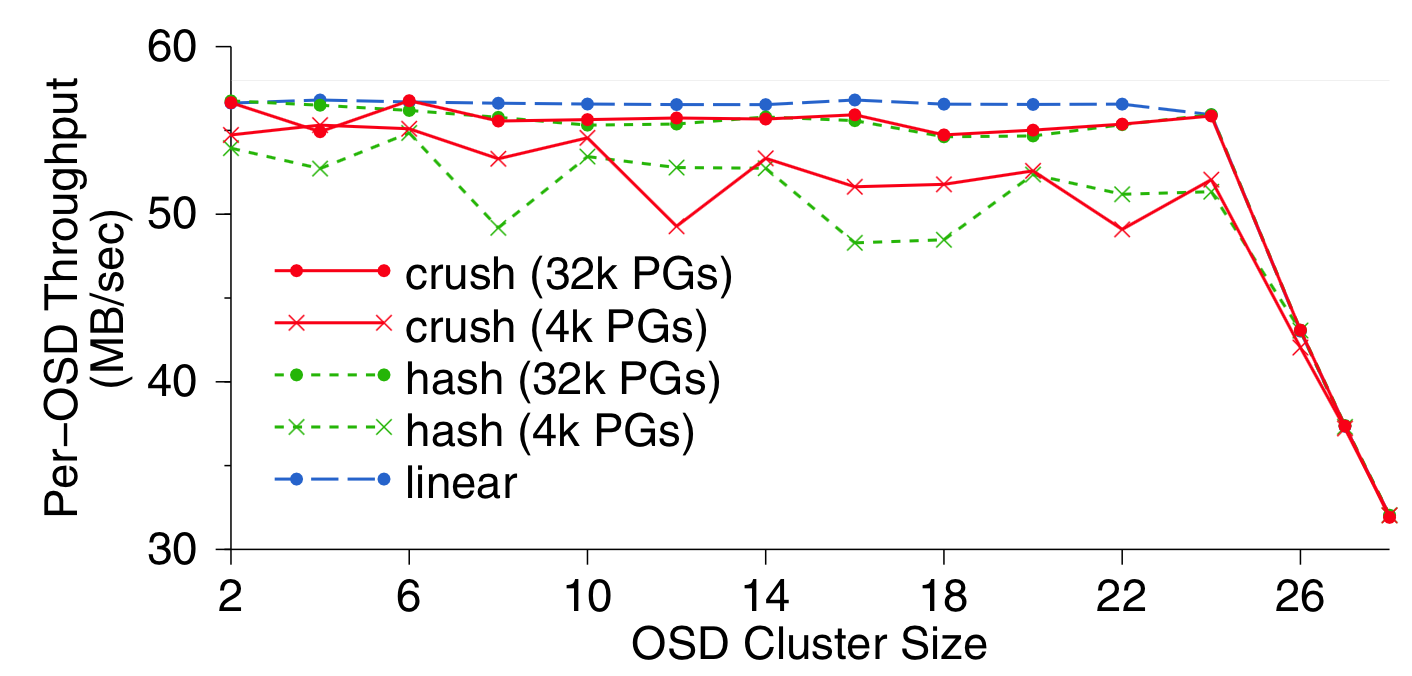
\includegraphics{figures/figure8.png}
\caption{Reprinting Figure 8 from the original paper {[}9{]}. The
original caption reads: ``\emph{object storage device (OSD) write
performance scales linearly with the size of the OSD cluster until the
switch is saturated at 24 OSDs. CRUSH and hash performance improves when
more PGs lower variance in OSD utilization}.''}
\end{figure}

\section{Discussion}\label{discussion}

We discuss different aspects of our proposal.

\subsection{Usability}\label{usability}

Given that the high-level components (\hyperref[sec:goals-means-obs]{})
abstract a large number of experiments that people usually implement in
the storage systems literature and since this is what a researcher
usually goes through anyway, creating the specification for an
experiment represents little extra effort. The exception being
documenting the experiment means which, as we mentioned before
(\hyperref[sec:means]{}), is a task that can be automated using
currently available tools.

\subsection{Integration into Existing
Infrastructure}\label{integration-into-existing-infrastructure}

Experimental platforms such as CloudLab {[}10{]} can incorporate the
notion of \emph{execution} so that for every experiment a record of
executions is maintained. For each execution, the means section of the
ESF can be automatically populated. Validation statements can also
provide another testability layer for continuous integration (CI)
systems such as Jenkins.

\subsection{Codified Observations As Falsifiable
Statements}\label{codified-observations-as-falsifiable-statements}

Validation clauses serve to succinctly codify observations. Given the
descriptive language design, validation ranges have to be provided for
each observation so that it can be tested. This has the implication of
turning observations into falsifiable statements {[}11{]}. These
validation clauses are conditions that should hold in order to
corroborate the conclusions of the paper. In other words, if the means
of the experiment are properly recreated, the specified behavior should
be observed.

\begin{figure}[htbp]
\centering
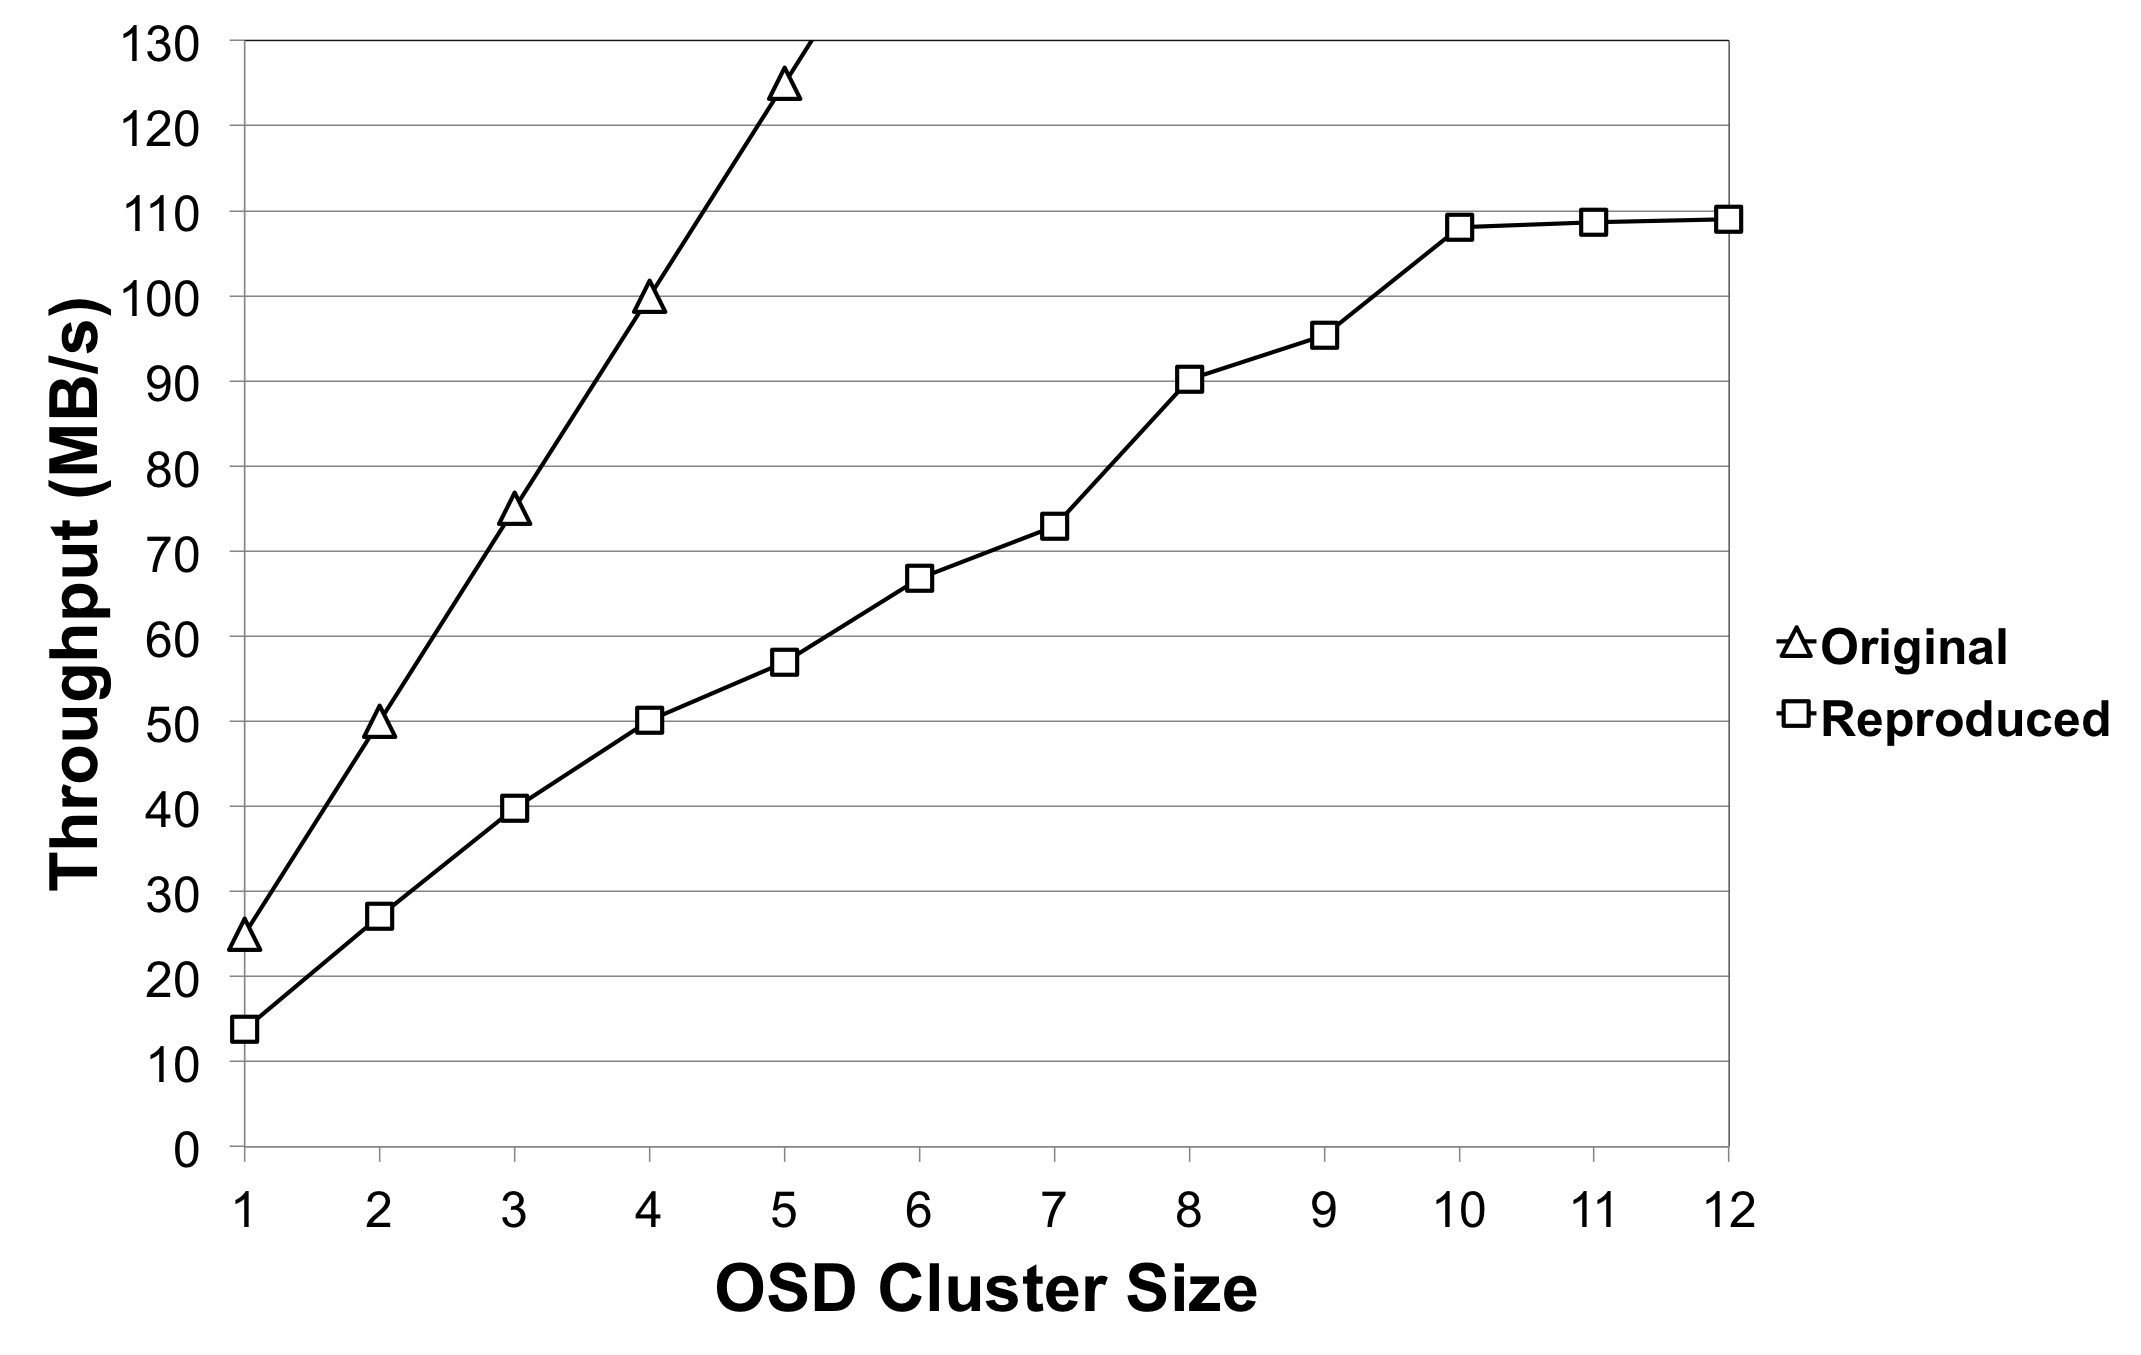
\includegraphics{figures/ceph.png}
\caption{Reproducing a scaled-down version of the original OSDI '06
scalability experiment. The x-axis corresponds to the size of the
cluster (in number of OSDs). The y-axis represents normalized throughput
(to meaningfully compare against original results) with respect to the
raw performance of the hard disk drives in the cluster. The red line
corresponds to the original results and the green line to the one
generated by the re-execution of the experiment.}
\end{figure}

Experiment goals (\hyperref[sec:goals]{}) set the tone in which these
falsifiable statements are treated. For an experiment that proves a
concept or design, a validation clause has more weight than, say, an
experiment that quantifies an expected overhead. For example, for a
system that claims to achieve linear scalability, the corresponding
validation clauses are more significant than those for an experiment
that shows the overhead of a new file system implemented as a FUSE
module. In the former, a failed validation invalidates the whole work
while in the latter the failed test invalidates a minor aspect. In other
words, some experiments evaluate a high-level claim while others refer
to low-level aspects, hence the importance of looking at experiment
goals while looking at validations; goals set the mindset of the reader
or reviewer that validates the work whenever she encounters failed
validations. This is the main motivation for having goals as an explicit
entry on the ESF.

\subsection{The Validation Workflow}\label{sec:workflow}

The ESF has the structure of a conditional statement: given the goals
and means of an experiment, the observations on the output data should
hold. Thus, if the validation statements are false with respect to the
output data of the re-execution of an experiment, it is either because
the differences between the means of the original and reproduced
experiment are significantly different, or the original claims cannot be
corroborated. Thus, before one can determine the latter, one has to
audit the differences between the means of experimentation and account
for all of them (Figure 4).

\begin{figure}[htbp]
\centering
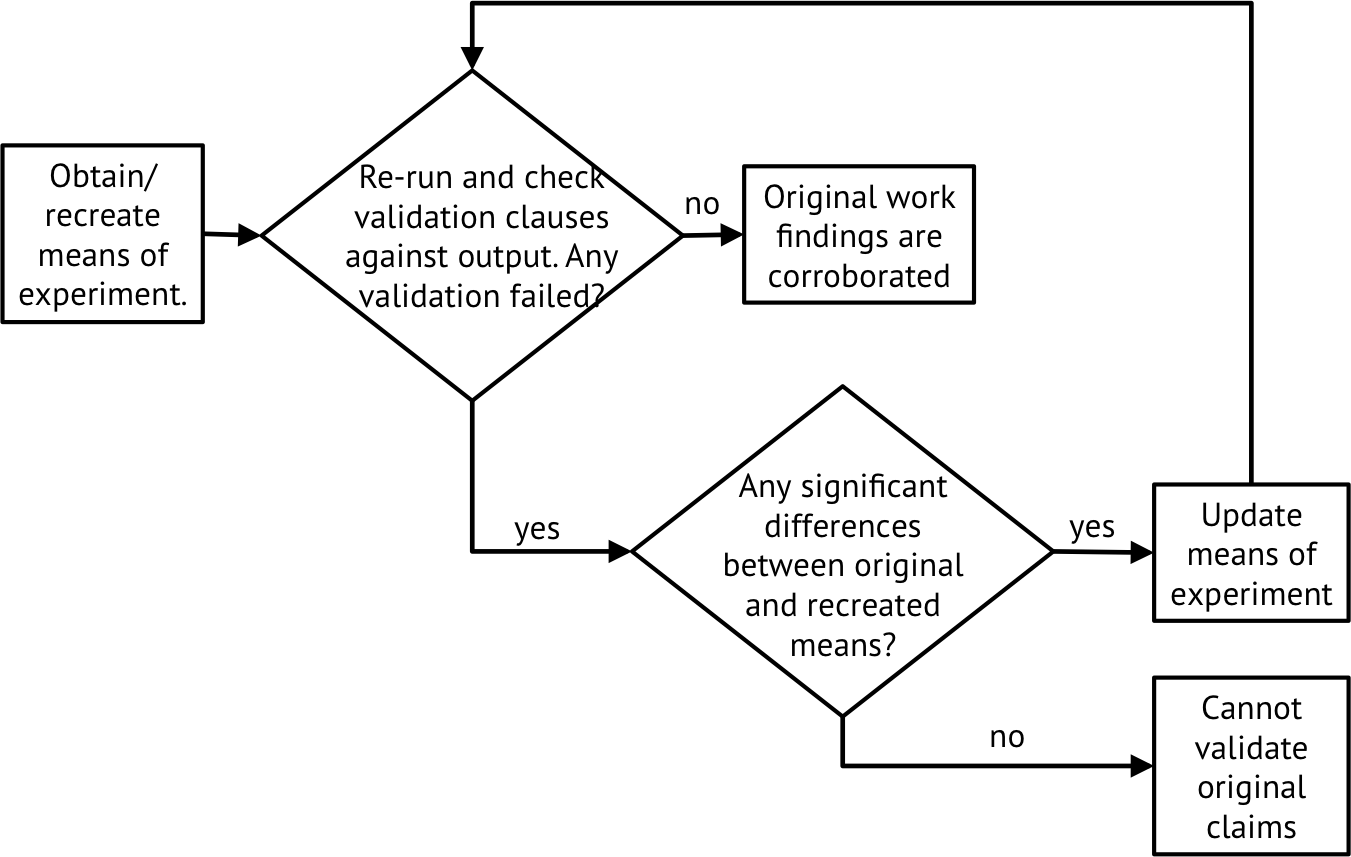
\includegraphics{figures/workflow.png}
\caption{Validation workflow.}
\end{figure}

\subsection{Early Feedback}\label{early-feedback}

The following are quotes from authors that have kindly worked with us by
creating specifications for one or more of their published experiments:

\begin{quote}
Author 1: \emph{Writing an experiment specification makes you think
clearly about the overall experiment design}.
\end{quote}

\begin{quote}
Author 2: \emph{The ESF provides a nice template for carrying out
experiments}.
\end{quote}

\begin{quote}
Author 3: \emph{This approach helps to find meaningful baselines.
Reporting raw numbers in figures and observations makes it harder to
validate results. Specifying validation clauses respective to baselines
and normalized values makes it easier to report reproducible results}.
\end{quote}

In general, we have noticed that the exercise of explicitly specifying
the validation criteria creates a feedback loop in an author's mind that
results in insightful ideas for experiment design, baseline selection,
and validation criteria. Additionally, the author's point of view is
explicitly expressed. Usually, figures contain more information than
necessary to back a claim. This which might lead readers to draw other
conclusions. Lastly, every article has an implicit temporal context
associated to it that the reader has to keep in mind, for example, the
bottleneck at the time that an article was published might be in storage
devices (e.g., hard disk drives) while at other times they might have
moved to the network instead (e.g., because of the availability of
faster storage devices such as SSDs). A possibility would be to create a
community-maintained knowledge base that an author can link the paper to
so that a semantic context is available to the reader.

\section{Related Work}\label{sec:related}

The challenging task of evaluating experimental results in applied
computer science has been long recognized {[}12--14{]}. This and other
related issues have gained substantial attention lately in systems
research {[}1,3,15--20{]}, computational science {[}17,18,21,22{]} and
science in general {[}23--25{]}. Similarly, efforts such as \emph{The
Recomputation Manifesto} {[}26{]} and the \emph{Software Sustainability
Institute} {[}27{]} have reproducibility as a central part of their
endeavour but leave performance as a secondary problem. In systems
research, performance \emph{is} the subject of study, thus we need to
look at it as a primary issue.

In {[}3{]} the authors took 601 articles published in 13 top-tier
systems research conferences and found that 32.3\% of associated
experiments are repeatable (under their definition of \emph{weak
repeatability}). The authors did not validate the original results. In
our case, we are interested not only in being able to rebuild and
execute binaries (repeat/reproduce the execution) but also in validating
the original claims by testing falsifiable statements on the output of
the experiment.

Krishnamurthi and Vitek {[}4{]} emphasize the importance of
repeatability and describe recent efforts by the systems research
community to encourage the submission of experiment artifacts as assets
associated to an article. We see our work as complementary to these
since an experiment specification could also be part of this list of
assets, making it easier to validate a re-generated result.

\section{Conclusion and Future Work}\label{conclusion-and-future-work}

In the words of Karl Popper: ``\emph{the criterion of the scientific
status of a theory is its falsifiability, or refutability, or
testability}''. By providing a way to specify the high-level components
of an experiment and validation clauses for observed metrics we
effectively incorporate falsifiability to the field of experimental
storage systems. We are in the process of studying the viability of the
ESF on experiments from other areas of systems research. As part of our
work, we are working with colleagues in our field to create descriptions
for already-published experiments and analyze them to check if they
capture the appropriate validation criteria. While we envision our
findings to be applicable in the area of systems research, we plan to
evaluate its suitability on other areas of computer science.

\textbf{Acknowledgements:} This work was performed under the auspices of
the U.S. Department of Energy by Lawrence Livermore National Laboratory
under Contract DE-AC52-07NA27344. LLNL-CONF-669866-DRAFT. Sandia
National Laboratories is a multi-program laboratory managed and operated
by Sandia Corporation, a wholly owned subsidiary of Lockheed Martin
Corporation, for the U.S. Department of Energy's National Nuclear
Security Administration under contract DE-AC04-94AL85000.

\section{References}\label{references}

\noindent
\vspace{-2em} \setlength{\parindent}{-0.26in}
\setlength{\leftskip}{0.2in} \setlength{\parskip}{8pt}

{[}1{]} J. Vitek and T. Kalibera, ``Repeatability, reproducibility, and
rigor in systems research,'' \emph{Proceedings of the ninth ACM
international conference on embedded software}, New York, NY, USA: ACM,
2011, pp. 33--38.

{[}2{]} C.T. Brown, ``How we make our papers replicable,'' 2014.
\url{http://ivory.idyll.org/blog/2014-our-paper-process.html}.

{[}3{]} C. Collberg, T. Proebsting, and A.M. Warren, ``Repeatability and
benefaction in computer systems research,'' 2015.

{[}4{]} S. Krishnamurthi and J. Vitek, ``The real software crisis:
Repeatability as a core value,'' \emph{Commun. ACM}, vol. 58, Feb. 2015,
pp. 34--36.

{[}5{]} B. Clark, T. Deshane, E. Dow, S. Evanchik, M. Finlayson, J.
Herne, and J.N. Matthews, ``Xen and the art of repeated research,''
\emph{Proceedings of the annual conference on USENIX annual technical
conference}, Berkeley, CA, USA: USENIX Association, 2004, pp. 47--47.

{[}6{]} I. Jimenez, C. Maltzahn, J. Lofstead, A. Moody, K. Mohror, R.H.
Arpaci-Dusseau, and A. Arpaci-Dusseau, ``The role of container
technology in reproducible computer systems research,''
\emph{Proceedings of the 4th international conference on cloud computing
engineering}, Tempe, AZ: 2015.

{[}7{]} F. Chirigati, D. Shasha, and J. Freire, ``ReproZip: Using
provenance to support computational reproducibility,'' \emph{Proceedings
of the 5th USENIX conference on theory and practice of provenance},
Berkeley, CA, USA: USENIX Association, 2013, pp. 1--1.

{[}8{]} I. Jimenez, C. Maltzahn, A. Moody, and K. Mohror, \emph{Redo:
Reproducibility at scale}, UC Santa Cruz, 2014.

{[}9{]} S.A. Weil, S.A. Brandt, E.L. Miller, D.D.E. Long, and C.
Maltzahn, ``Ceph: A scalable, high-performance distributed file
system,'' \emph{Proceedings of the 7th symposium on operating systems
design and implementation}, Berkeley, CA, USA: USENIX Association, 2006,
pp. 307--320.

{[}10{]} R. Ricci and E. Eide, ``Introducing CloudLab: Scientific
infrastructure for advancing cloud architectures and
applications,''\emph{;login:} vol. 39, Dec. 2014, pp. 36--38.

{[}11{]} K. Popper, \emph{The logic of scientific discovery}, New Delhi:
Routledge, 2002.

{[}12{]} J.P. Ignizio, ``On the establishment of standards for comparing
algorithm performance,'' \emph{Interfaces}, vol. 2, Nov. 1971, pp.
8--11.

{[}13{]} J.P. Ignizio, ``Validating claims for algorithms proposed for
publication,'' \emph{Operations Research}, vol. 21, May. 1973, pp.
852--854.

{[}14{]} H. Crowder, R.S. Dembo, and J.M. Mulvey, ``On reporting
computational experiments with mathematical software,'' \emph{ACM Trans.
Math. Softw.}, vol. 5, Jun. 1979, pp. 193--203.

{[}15{]} C. Dietrich and D. Lohmann, ``The dataref versuchung: Saving
time through better internal repeatability,'' \emph{SIGOPS Oper. Syst.
Rev.}, vol. 49, Jan. 2015, pp. 51--60.

{[}16{]} D.G. Feitelson, ``From repeatability to reproducibility and
corroboration,'' \emph{SIGOPS Oper. Syst. Rev.}, vol. 49, Jan. 2015, pp.
3--11.

{[}17{]} J. Freire, P. Bonnet, and D. Shasha, ``Computational
reproducibility: State-of-the-art, challenges, and database research
opportunities,'' \emph{Proceedings of the 2012 ACM SIGMOD international
conference on management of data}, New York, NY, USA: ACM, 2012, pp.
593--596.

{[}18{]} C. Neylon, J. Aerts, C.T. Brown, S.J. Coles, L. Hatton, D.
Lemire, K.J. Millman, P. Murray-Rust, F. Perez, N. Saunders, N. Shah, A.
Smith, G. Varoquaux, and E. Willighagen, ``Changing computational
research: The challenges ahead,'' \emph{Source Code for Biology and
Medicine}, vol. 7, Dec. 2012, pp. 1--2.

{[}19{]} R. LeVeqije, I. Mitchell, and V. Stodden, ``Reproducible
research for scientific computing: Tools and strategies for changing the
culture,'' \emph{Computing in Science Engineering}, vol. 14, Jul. 2012,
pp. 13--17.

{[}20{]} V. Stodden, F. Leisch, and R.D. Peng, \emph{Implementing
reproducible research}, CRC Press, 2014.

{[}21{]} R.D. Peng, ``Reproducible research in computational science,''
\emph{Science}, vol. 334, Dec. 2011, pp. 1226--1227.

{[}22{]} D.L. Donoho, A. Maleki, I.U. Rahman, M. Shahram, and V.
Stodden, ``Reproducible research in computational harmonic analysis,''
\emph{Computing in Science \& Engineering}, vol. 11, Jan. 2009, pp.
8--18.

{[}23{]} J. Achenbach, ``The new scientific revolution: Reproducibility
at last,'' \emph{The Washington Post}, Jan. 2015.

{[}24{]} M.B. Yaffe, ``Reproducibility in science,'' \emph{Science
Signaling}, vol. 8, Apr. 2015, pp. eg5--eg5.

{[}25{]} Editorial, ``Journals unite for reproducibility,''
\emph{Nature}, vol. 515, Nov. 2014, pp. 7--7.

{[}26{]} I.P. Gent, ``The recomputation manifesto,''
\emph{arXiv:1304.3674 {[}cs{]}}, Apr. 2013.

{[}27{]} S. Crouch, N. Hong, S. Hettrick, M. Jackson, A. Pawlik, S.
Sufi, L. Carr, D. De Roure, C. Goble, and M. Parsons, ``The software
sustainability institute: Changing research software attitudes and
practices,'' \emph{Computing in Science Engineering}, vol. 15, Nov.
2013, pp. 74--80.

% letter {
% }

% a0poster {
% }
\end{document}
